\documentclass[11pt]{beamer}
\usepackage[utf8]{inputenc}
\usepackage[T1]{fontenc}
\usepackage{lmodern}
\usepackage{graphicx}
\usepackage{tikz}
\usepackage{apacite}
\usetikzlibrary{shapes.geometric, arrows.meta,positioning}
\usepackage[makeroom,thicklines,samesize]{cancel}
\usepackage[english]{babel}
\usepackage[percent]{overpic}
\usetheme{default}
\begin{document}
	\author{Paulina Friemann}
	\date{February 23, 2021}
	\title{Assessing biological and computational approaches to path-finding through inverse planning}
	%\subtitle{}
	%\logo{}
	%\institute{}
	%\date{}
	%\subject{}
	%\setbeamercovered{transparent}
	%\setbeamertemplate{navigation symbols}{}
	\begin{frame}[plain]
		\maketitle
	\end{frame}

	\begin{frame}
	\frametitle{How can we determine an agent's goal?}
\begin{overpic}[width=1.0\textwidth,tics=10]{res/ant_example_1}
	\put (20,85) {\huge$\displaystyle\gamma$}
\end{overpic}
	\end{frame}

	\begin{frame}
	\frametitle{Structure}
	\begin{itemize}
		\item Action understanding as inverse planning
		\item Model and computations
		\item Model flow
		\item Changes and plans
	\end{itemize}
\end{frame}

	\begin{frame}
	\frametitle{How can we determine an agent's goal?}
	\begin{overpic}[width=1.0\textwidth,tics=10]{res/ant_example_1}
		\put (27,20) {\LARGE$\displaystyle P = 0.5$}
		\put (70, 45) {\LARGE$\displaystyle P = 0.5$}
	\end{overpic}
\end{frame}


	\begin{frame}
	\frametitle{Predictions change with observations}
\begin{overpic}[width=1.0\textwidth,tics=10]{res/ant_example_2}
	\put (27,20) {\LARGE$\displaystyle P = 0.5$}
	\put (70, 45) {\LARGE$\displaystyle P = 0.5$}
\end{overpic}
	\end{frame}

	\begin{frame}
	\frametitle{Predictions change with observations}
	\begin{overpic}[width=1.0\textwidth,tics=10]{res/ant_example_2}
		\put (27,20) {\LARGE$\displaystyle P = \cancel{0.5}$}
		\put (70, 45) {\LARGE$\displaystyle P = \cancel{0.5}$}
	\end{overpic}
\end{frame}	

	\begin{frame}
	\frametitle{Predictions change with observations}
	\begin{overpic}[width=1.0\textwidth,tics=10]{res/ant_example_2}
		\put (27,20) {\LARGE$\displaystyle P = \cancel{0.5}$}
		\put (38,25) {\LARGE$\displaystyle 0.2$}
		\put (70, 45) {\LARGE$\displaystyle P = \cancel{0.5}$}
		\put (81,50) {\LARGE$\displaystyle 0.8$}
	\end{overpic}
\end{frame}	

\begin{frame}
	\frametitle{Action understanding as inverse planning}
	\framesubtitle{Baker, Saxe \& Tenenbaum, 2009}
	
	\begin{itemize}
		\item Goal: modeling human theory of mind
		\item 3 experiments: showing an agent moving in an abstract environment
	\end{itemize}
		\begin{figure}
	\centering
	\includegraphics[width=0.68\linewidth, trim=15pt 0pt 0pt 15pt, clip]{res/tenenbaum_exp}
	\caption{from \citeA{baker2009}}
\end{figure}
\end{frame}

\begin{frame}
	\frametitle{Action understanding as inverse planning}
	\framesubtitle{Baker, Saxe \& Tenenbaum, 2009}
	\begin{itemize}
		\item Participants were asked to judge likelihood of agent going to goals
		\item These judgments were correlated with model predictions
	\end{itemize}
\end{frame}

\begin{frame}
	\begin{figure}
		\centering
		\includegraphics[width=0.98\linewidth]{res/exp_results}
		\caption{(a) Stimuli (b) participants' ratings (c) model predictions  (from \citeA{baker2009})}
	\end{figure}
\end{frame}



\begin{frame}
	\frametitle{Action understanding as inverse planning}
	\framesubtitle{Baker, Saxe \& Tenenbaum, 2009}
	\begin{itemize}
		\item Modeling Theory of Mind
		\item Infer goal from observed actions
		\item Use Bayesian rule:
	\end{itemize}
\vspace*{2em}
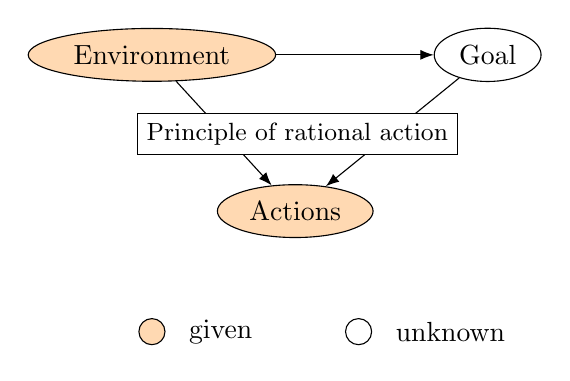
\begin{tikzpicture}
	\node[draw, ellipse, fill=orange!30] (env) {Environment};
	\node[draw, ellipse, right=2cm of env] (goal) {Goal};
	\node[draw, ellipse, fill=orange!30, below right=1.5cm and .cm of env] (act) {Actions};
	\draw[-{Latex}] (env) -- (goal);
	\draw[-{Latex}] (env) -- (act);
	\draw[-{Latex}] (goal) -- (act);
	\node[draw, ellipse, fill=orange!30, below=3cm of env] (given) {};
	\node[right=.5em of given] (givent) {given};
	\node[draw, ellipse,right=3em of givent] (unknown) {};
	\node[right=.5em of unknown] (unknownt) {unknown};
	\node[draw, below left=.5cm and -5cm of env, fill=white] (hello) {{\small Principle of rational action}};
\end{tikzpicture}
\end{frame}


\begin{frame}
	\frametitle{Action understanding as inverse planning}
	\framesubtitle{Baker, Saxe \& Tenenbaum, 2009}
	
	Steps to goal prediction:
	\begin{enumerate}
		\item Setup: Specify Environment, Goals, Obstacles
		\item Planning Phase: Model policies to goals
		\item Observation Phase:
		\begin{itemize}
			\item Observe movement OR
			\item Sample movement
		\end{itemize}
		\item Inference Phase:
		Apply Bayes rule
	\end{enumerate}
\end{frame}

\begin{frame}
	\frametitle{1: Setup}
	\begin{columns}
		\begin{column}{0.7\textwidth}
				\begin{overpic}[width=0.95\textwidth,tics=10]{res/ant_step1_ob}
		\end{overpic}
	\end{column}
		\begin{column}{0.3\textwidth}
	\begin{overpic}[width=1.0\textwidth,tics=10]{res/legend}
	\end{overpic}
\end{column}
	\end{columns}
\end{frame}

\begin{frame}
	\frametitle{2: Planning Phase}
	\begin{overpic}[width=0.48\textwidth,tics=10]{res/ant_step2b_obs}
	\end{overpic}
	\begin{overpic}[width=.48\textwidth,tics=10]{res/ant_step2_obs}
	\end{overpic}
\end{frame}

\begin{frame}
	\frametitle{2: Planning Phase}
	\framesubtitle{Plans vs policies}
	\begin{columns}
		\begin{column}{0.5\textwidth}
			Plan:
			\vspace*{1em}
			%\begin{center}
			
				\begin{overpic}[width=0.8\textwidth,tics=10]{res/ant_plan}
				\end{overpic}
				
			%\end{center}
		$\rightarrow$ Sequence of actions
		\end{column}
		\begin{column}{0.5\textwidth}  %%<--- here
			Policy:
			\vspace*{1em}
			%\begin{center}
			
				\begin{overpic}[width=0.8\textwidth,tics=10]{res/ant_step2b_obs}
				\end{overpic}
			
			%\end{center}
		$\rightarrow$ Mapping from states to actions
		\end{column}
	\end{columns}
\end{frame}

\begin{frame}
	\frametitle{2: Planning Phase}
	\framesubtitle{Markov Decision Problems}
	\begin{itemize}
		\item Finding optimal strategies
		\item Stochastic actions $\rightarrow$ state transitions can be non-deterministic
		\item \textit{Markov Property}: Transition probabilities only depend on the current state
	\end{itemize}
\vspace*{2em}
In \citeA{baker2009}:\\%Baker, Saxe \& Tenenbaum (2009): \\
Transitions are deterministic, but decisions are stochastic\\
$\rightarrow$ agent doesn't always choose the optimal action
	
\end{frame}

\begin{frame}
	\frametitle{2: Planning Phase}
	\framesubtitle{Solving MDPs: e.g. \textit{Value Iteration }algorithm}
	States S, actions A, goals G, obstacles O, transition model $T_{i,a,j}$\\
	\vspace*{1em}
	\begin{enumerate}
		\item Reward function for all $i,j \in$ S that are connected with an action $a \in$ A, given a goal $g$: 
		\begin{equation*}
			R(i,a,j | g)= 
			\begin{cases}
				\text{goal reward} + \text{move cost}(a)& \text{if } i = g\\
				\text{trap cost}              & \text{if } i \in O \\
				\text{move cost}(a) & \text{else}
			\end{cases}
		\end{equation*}
	\item Utility function for all i $\in$ S, given goal g (and a discount factor $\gamma$):
	\begin{equation*}
		U_{t+1}(i|g) \leftarrow \underset{a}{\max} ( R(i,a,j|g) + \gamma U_t(j|g)  ), ~~~a,j \in T_i
	\end{equation*}
	\end{enumerate}	
\end{frame}

\begin{frame}
	\frametitle{2: Planning Phase}
	\framesubtitle{Solving MDPs: e.g. \textit{Value Iteration }algorithm}
	
	\begin{enumerate}
		\setcounter{enumi}{2}
		\item Given a determinism factor $\beta$, calculate goal-dependent policies by taking the soft-max of the utilities:
		%\[
		\begin{equation*}
			\setcounter{enumi}{3}
			P_\pi(a|i,g) = \frac{exp(  \beta(  R(i,a,j|g) + \gamma U(j|g)  )  )}{ \sum_{T_i}  exp(  \beta(  R(i,a,j|g) + \gamma U(j|g)  )  )}
		\end{equation*}
		%\]
		for all $a,j \in T_i$. 
	\end{enumerate}

	
\end{frame}

\begin{frame}
	\frametitle{3: Observation Phase}
	\begin{overpic}[width=1.0\textwidth,tics=10]{res/ant_step3_obs}
	\end{overpic}
\end{frame}

\begin{frame}
	\frametitle{4: Inference Phase}
	\begin{overpic}[width=1.0\textwidth,tics=10]{res/ant_step4}
	\end{overpic}
\end{frame}


\begin{frame}
	\frametitle{4: Inference Phase}
	Calculate probability of trajectory recursively:
	\begin{flalign*}
		& P(s_0|G=g) = P(g) \\
		& P(s_0, s_1 | G=g) = P(s_0 | G=g) \cdot P_\pi(a | s_0, g) \\
		& ... \\
		& P(s_0, ...,s_T | G=g) = P(s_0,...,s_{T-1} | G=g) \cdot P_\pi(a | s_{T-1}, g)
		\vspace*{2em}
	\end{flalign*}
\newline
Likelihood of each goal using Bayes' rule:
\begin{equation*}
	P(g|s_1,...,s_T) \propto P(s_2,...,s_T|s_1, g) \cdot P(g)
\end{equation*} 
	
\end{frame}

\begin{frame}
	\frametitle{Program Flow}
	\framesubtitle{Environment Specification}
	
\begin{figure}
	\centering
	\includegraphics[width=\linewidth]{res/env}
\end{figure}
\end{frame}

\begin{frame}
	\frametitle{Program Flow}
	\framesubtitle{Reward Function}
	
\begin{figure}
	\centering
	\includegraphics[width=\linewidth]{res/A_reward}
\end{figure}
\end{frame}

\begin{frame}
	\frametitle{Program Flow}
	\framesubtitle{Utilitiy Function}

\begin{figure}
	\centering
	\includegraphics[width=\linewidth]{res/A_utilities}
\end{figure}
\end{frame}

\begin{frame}
	\frametitle{Program Flow}
	\framesubtitle{Policies}
	\begin{figure}
		\centering
		\includegraphics[width=\linewidth]{res/A_policies}
	\end{figure}
	
\end{frame}

\begin{frame}
	\frametitle{Program Flow}
	\framesubtitle{Reward Function}
	\begin{figure}
		\centering
		\includegraphics[width=\linewidth]{res/B_reward}
	\end{figure}
\end{frame}

\begin{frame}
	\frametitle{Program Flow}
	\framesubtitle{Utility Function}
	\begin{figure}
		\centering
		\includegraphics[width=\linewidth]{res/B_utilities}
	\end{figure}
\end{frame}

\begin{frame}
	\frametitle{Program Flow}
	\framesubtitle{Policies}
	\begin{figure}
		\centering
		\includegraphics[width=\linewidth]{res/B_policies}
	\end{figure}
	
\end{frame}

\begin{frame}
	\frametitle{Program Flow}
	\framesubtitle{Trajectory Sampling}
	\begin{figure}
		\centering
		\includegraphics[width=\linewidth]{res/traj}
	\end{figure}
	
\end{frame}

\begin{frame}
	\frametitle{Program Flow}
	\framesubtitle{Posteriors}
	
\begin{figure}
	\centering
	\includegraphics[width=0.7\linewidth]{res/posteriors_m1}
\end{figure}

\begin{figure}
	\centering
	\includegraphics[width=0.7\linewidth]{res/posteriors_m2}
\end{figure}

\end{frame}

\begin{frame}
	\frametitle{Changes and Plans}
	\begin{itemize}
		\item A general evaluation of path-finding methods as models of natural agent navigation:
		\begin{itemize}
		\item[a)] Theoretical evaluation of run time and memory complexity, assumptions, restrictions, etc.
		\item[b)] Simulation-based evaluation
	\end{itemize}
	\item Relating AI methods and representations to natural counterparts
	\item Proposing new experiments 
	\end{itemize}
\end{frame}

% todo distance direction
\begin{frame}
	\frametitle{Changes and Plans}
	%\framesubtitle{Changes}
	\begin{enumerate}
		\item Setup: Specify Environment, Goals, Obstacles
		\item \textbf{{\Large Planning Phase}}: Model policies to goals
		\item Observation Phase:
		\begin{itemize}
			\item Observe movement OR
			\item Sample movement
		\end{itemize}
		\item \textbf{{\Large Inference Phase}}:
		Apply Bayes rule
	\end{enumerate}
\end{frame}

\begin{frame}
	\frametitle{Planning Phase}
	\begin{itemize}
		\item Representations
		\begin{itemize}
			\item Map-like
			\item Vectors / Distance and directions
			\item Hierarchical
			\item Omniscient vs limited
			\item ...
		\end{itemize}
		\item Calculations
		\begin{itemize}
			\item Random Walk
			\item Exhaustive Search
			\item Informed Search
			\item ...
		\end{itemize}
	\end{itemize}
	Depending on specific problems and combinations, these can be showing as the same empirically.
\end{frame}

\begin{frame}
	\frametitle{Inference Phase}
	\begin{itemize}
		\item Right now inferences to goals
		\item Calculate likelihood of models
		\item inferences to "mental states"
	\end{itemize}
\end{frame}

\begin{frame}
	\frametitle{Issues and Questions}
	\begin{itemize}
		\item Planning, policies and reactivity
		\item What is biological plausibility?
		\item Representations
		\item Other factors that drive navigation?
		\item Dependence of empirical results on combination of representation type and computations
	\end{itemize}
\end{frame}

\bibliographystyle{apacite}

\setlength{\bibleftmargin}{.125in}
\setlength{\bibindent}{-\bibleftmargin}

\begin{frame}
	\frametitle{Literature}
	\bibliography{../pathfinding.bib}
\end{frame}



\end{document}